\documentclass[12pt]{article}
\usepackage[utf8]{inputenc}
\newenvironment{sol}[1][Solution]{\begin{trivlist}\item[\hskip\labelsep {\bfseries #1:}]}{\end{trivlist}}
\usepackage[margin=1in]{geometry} 
\usepackage{amsmath,amsthm,amssymb}
\usepackage{color}
\usepackage{minted}
\usepackage{graphicx}
\title{Southern Methodist University \\
Bobby B. Lyle School of Engineering Department of Computer Science \\
Homework 5
}
\usepackage{times,url}   
\author{Operating System and Software System \\
Name: Bingying Liang 
\\ ID: 48999397\\ 
Email: bingyingl@smu.edu \\ 
CS7343 Distance}
\date{Feb 28 2023}

\begin{document}
\maketitle
\begin{itemize}
    \item CS 5343 students must answer exactly 2 projects
    \item CS 7343 students must answer all projects
\end{itemize}
    \begin{enumerate}
        \item \textbf{Project 2—The Sleeping Teaching Assistant (Chapter 7, P-38)}
        \item \textbf{Project 3—The Dining-Philosophers Problem (Chapter 7, P-39) }
        \item \textbf{Project 4—The Producer – Consumer Problem (Chapter 7, P-40)}
    \end{enumerate}
    For each project, please submit 
    \begin{enumerate}
        \item The source code of the project
        \item Brief description of how to test your program
        \item A sample Output
    \end{enumerate}
    All of the above should be place on folder (called Project1 \& Project2). These two folders should be placed in a folder bearing your name (e.g., Mike Smith). The folder “Mike Smith” should be zipped and uploaded to Canvas. 
    
    \newpage
    \section*{Environment}
    Laptop: MacBook Air M2 2022, macOS 13.3\\
    
    Programming APP: CLion 2022.2.3 \\
    
    Runtime version: 17.0.4+7-b469.53 aarch64\\
    
    VM: OpenJDK 64-Bit Server VM by JetBrains s.r.o.\\
    
    GC: G1 Young Generation, G1 Old Generation\\
    
    Memory: 2000M\\
    
    Cores: 8\\
    
    Running: Ubuntu 22.04 ARM64 Parallels Desktop as virtual environment.\\
    
    \newpage
    \section*{Project 2--The sleeping Teaching Assistant}
    
    A university computer science department has a teaching assistant (TA) who helps undergraduate students with their programming assignments during regular office hours. The TA's office is rather small and has room for only one desk with a chair and computer. There are three chairs in the hallway outside the office where students can sit and wait if the TA is currently helping another student. When there are no students who need help during office hours, the TA sits at the desk and takes a nap. If a student arrives during office hours and finds the TA sleeping, the student must awaken the TA to ask for help. If a student arrives and finds the TA currently helping another student, the student sits on one of the chairs in the hallway and waits. If no chairs are available, the student will come back at a later time.\\
    Using POSIX threads, mutex locks, and semaphores, implement a solution that cooridnates the activities of the TA and the students. Details for this assignment are provided below.
    \subsection*{The Students and the TA}
    Using Pthreads(Section 4.4.1), begin by creating $n$ students where each student will run as a separate thread. The TA will run as a separate thread as well. Students thread will alternate between programming for a period of time and seeking help from the TA. If the TA is available, they will obtain help. Otherwise, they will either sit in a chair in the hallway or, if no chairs are available, will resume programming and will seek help at a later time. If a student arrives and notices that the TA is sleeping, the student must notify the TA using a semaphore. When the TA finishes helping a student, the TA must check to see if there are students waiting for help in the hallway. If so, the TA must help each of these students in turn. If no students are present, the TA may return to napping.\\
    Perhaps the best option for simulating students programming -- as well as the TA providing help to a student -- is to have the appropriate threads sleep for a random period of time.
    Coverage of POSIX mutex locks and semaphores is provided Section 7.3. Consult that section for details.

    \begin{sol}
    \hspace*{\hill}
        \begin{minted}[frame=lines,framesep=2mm,baselinestretch=1.2,fontsize=\footnotesize,linenos]{c}
// Created by Eve Liang on 3/26/23.
#include <stdio.h>
#include <stdlib.h>
#include <unistd.h>
#include <string.h>
#include <pthread.h>
#include <semaphore.h>
#include <sys/time.h>

int ta_teaching_time;
int s_visit_time;
int s_leave_time;

int chair_num;
int ta_num;
int student_num;

sem_t student_sem;
sem_t ta_sem;

sem_t mutex;
sem_t s_mutex;
sem_t t_mutex;

int i, j, k;

int working_ta = 1;
int waiting_students = 0;

int leave_cnt = 0;
int served_cnt = 0;
int ta_serve_cnt[50] = {0};
void msleep(int tms);

void set_useed(){
    struct timeval tv;
    gettimeofday(&tv, NULL);
    srand(tv.tv_sec + tv.tv_usec);
}
void *TA(void *tid_){
    while (1)
    {
        set_useed();
        long tid = (long)tid_;

        sem_wait(&student_sem);
        sem_wait(&mutex);
        waiting_students--;
        printf("TA start teaching.\n");
        printf("The number of waiting students: %d\n", waiting_students);
        sem_post(&mutex);
        set_useed();
        ta_teaching_time = rand() % 1001;
        msleep(ta_teaching_time);

        int current_served_cnt;
        sem_wait(&t_mutex);
        served_cnt++;
        current_served_cnt = served_cnt;
        ta_serve_cnt[tid]++;
        sem_post(&t_mutex);

        printf("%dth arrived student finishes.", current_served_cnt);
        printf("This time TA service time is: %d\n", ta_teaching_time);
        sem_post(&ta_sem);
        printf("TA if no students will sleep\n");

    }
}

void *student(void *sid_){
    s_leave_time = rand() % 21;
    long sid = (long)sid_;
    printf("%ldth students come here\n", sid);

    sem_wait(&mutex);    // for waiting_students
    sem_wait(&s_mutex);

    if (waiting_students == chair_num){
        leave_cnt++;

        printf("There is no seats, %ldth student leave:%d\n", sid, leave_cnt);
        /* free mutexes */
        sem_post(&s_mutex);
        sem_post(&mutex);
    }
    else{
        waiting_students++;
        printf("%ldth student has chair, sit down. The waiting student number is:%d\n", sid, waiting_students);

        int student_value;

        /* free mutexes */
        sem_post(&s_mutex);
        sem_post(&mutex);

        sem_post(&student_sem);

        sem_wait(&ta_sem);
    }

    msleep(s_leave_time);
}

void msleep(int tms){
    struct timeval tv;

    tv.tv_sec = tms / 1000;
    tv.tv_usec = (tms % 1000) * 1000;
    select(0, NULL, NULL, NULL, &tv);
}

int main(int argc, char *argv[]){

    chair_num = 4; // one in office, the other three hallway
    ta_num = 1;

    student_num = atoi(argv[1]);

    if (argc != 2){
        fprintf(stderr, "Please use the command format: <file> <number of students>");
    }

    pthread_t ta_thread[ta_num], student_thread[student_num];

    sem_init(&ta_sem, 0, 0);
    sem_init(&student_sem, 0, 0);

    sem_init(&mutex, 0, 1);
    sem_init(&s_mutex, 0, 1);
    sem_init(&t_mutex, 0, 1);


    for (i = 1; i <= ta_num; i++)
    {
        pthread_create(&ta_thread[i], NULL, TA, (void *) (long) (i));
    }

    for (i = 1; i <= student_num; i++)
    {
        s_visit_time = rand() % 500000 / 2;
        printf("(create)student_visit_time:%d,usleeping...\n", s_visit_time);
        usleep(s_visit_time);
        pthread_create(&student_thread[i], NULL, student, (void *) (long) (i));

    }

    for (i = 1; i <= student_num; i++)
    {
        pthread_join(student_thread[i], NULL);
    }

    printf("All students has finished. TA sleep\n");

    return 0;

}

        \end{minted}
    
        \textbf{The result}
    \begin{minted}[frame=lines,framesep=2mm,baselinestretch=1.2,fontsize=\footnotesize]{c}
 ./<filename> <The numbers of students>
    \end{minted}
    The result for running of each philosopher only eating one times and two times.
    \begin{center}
        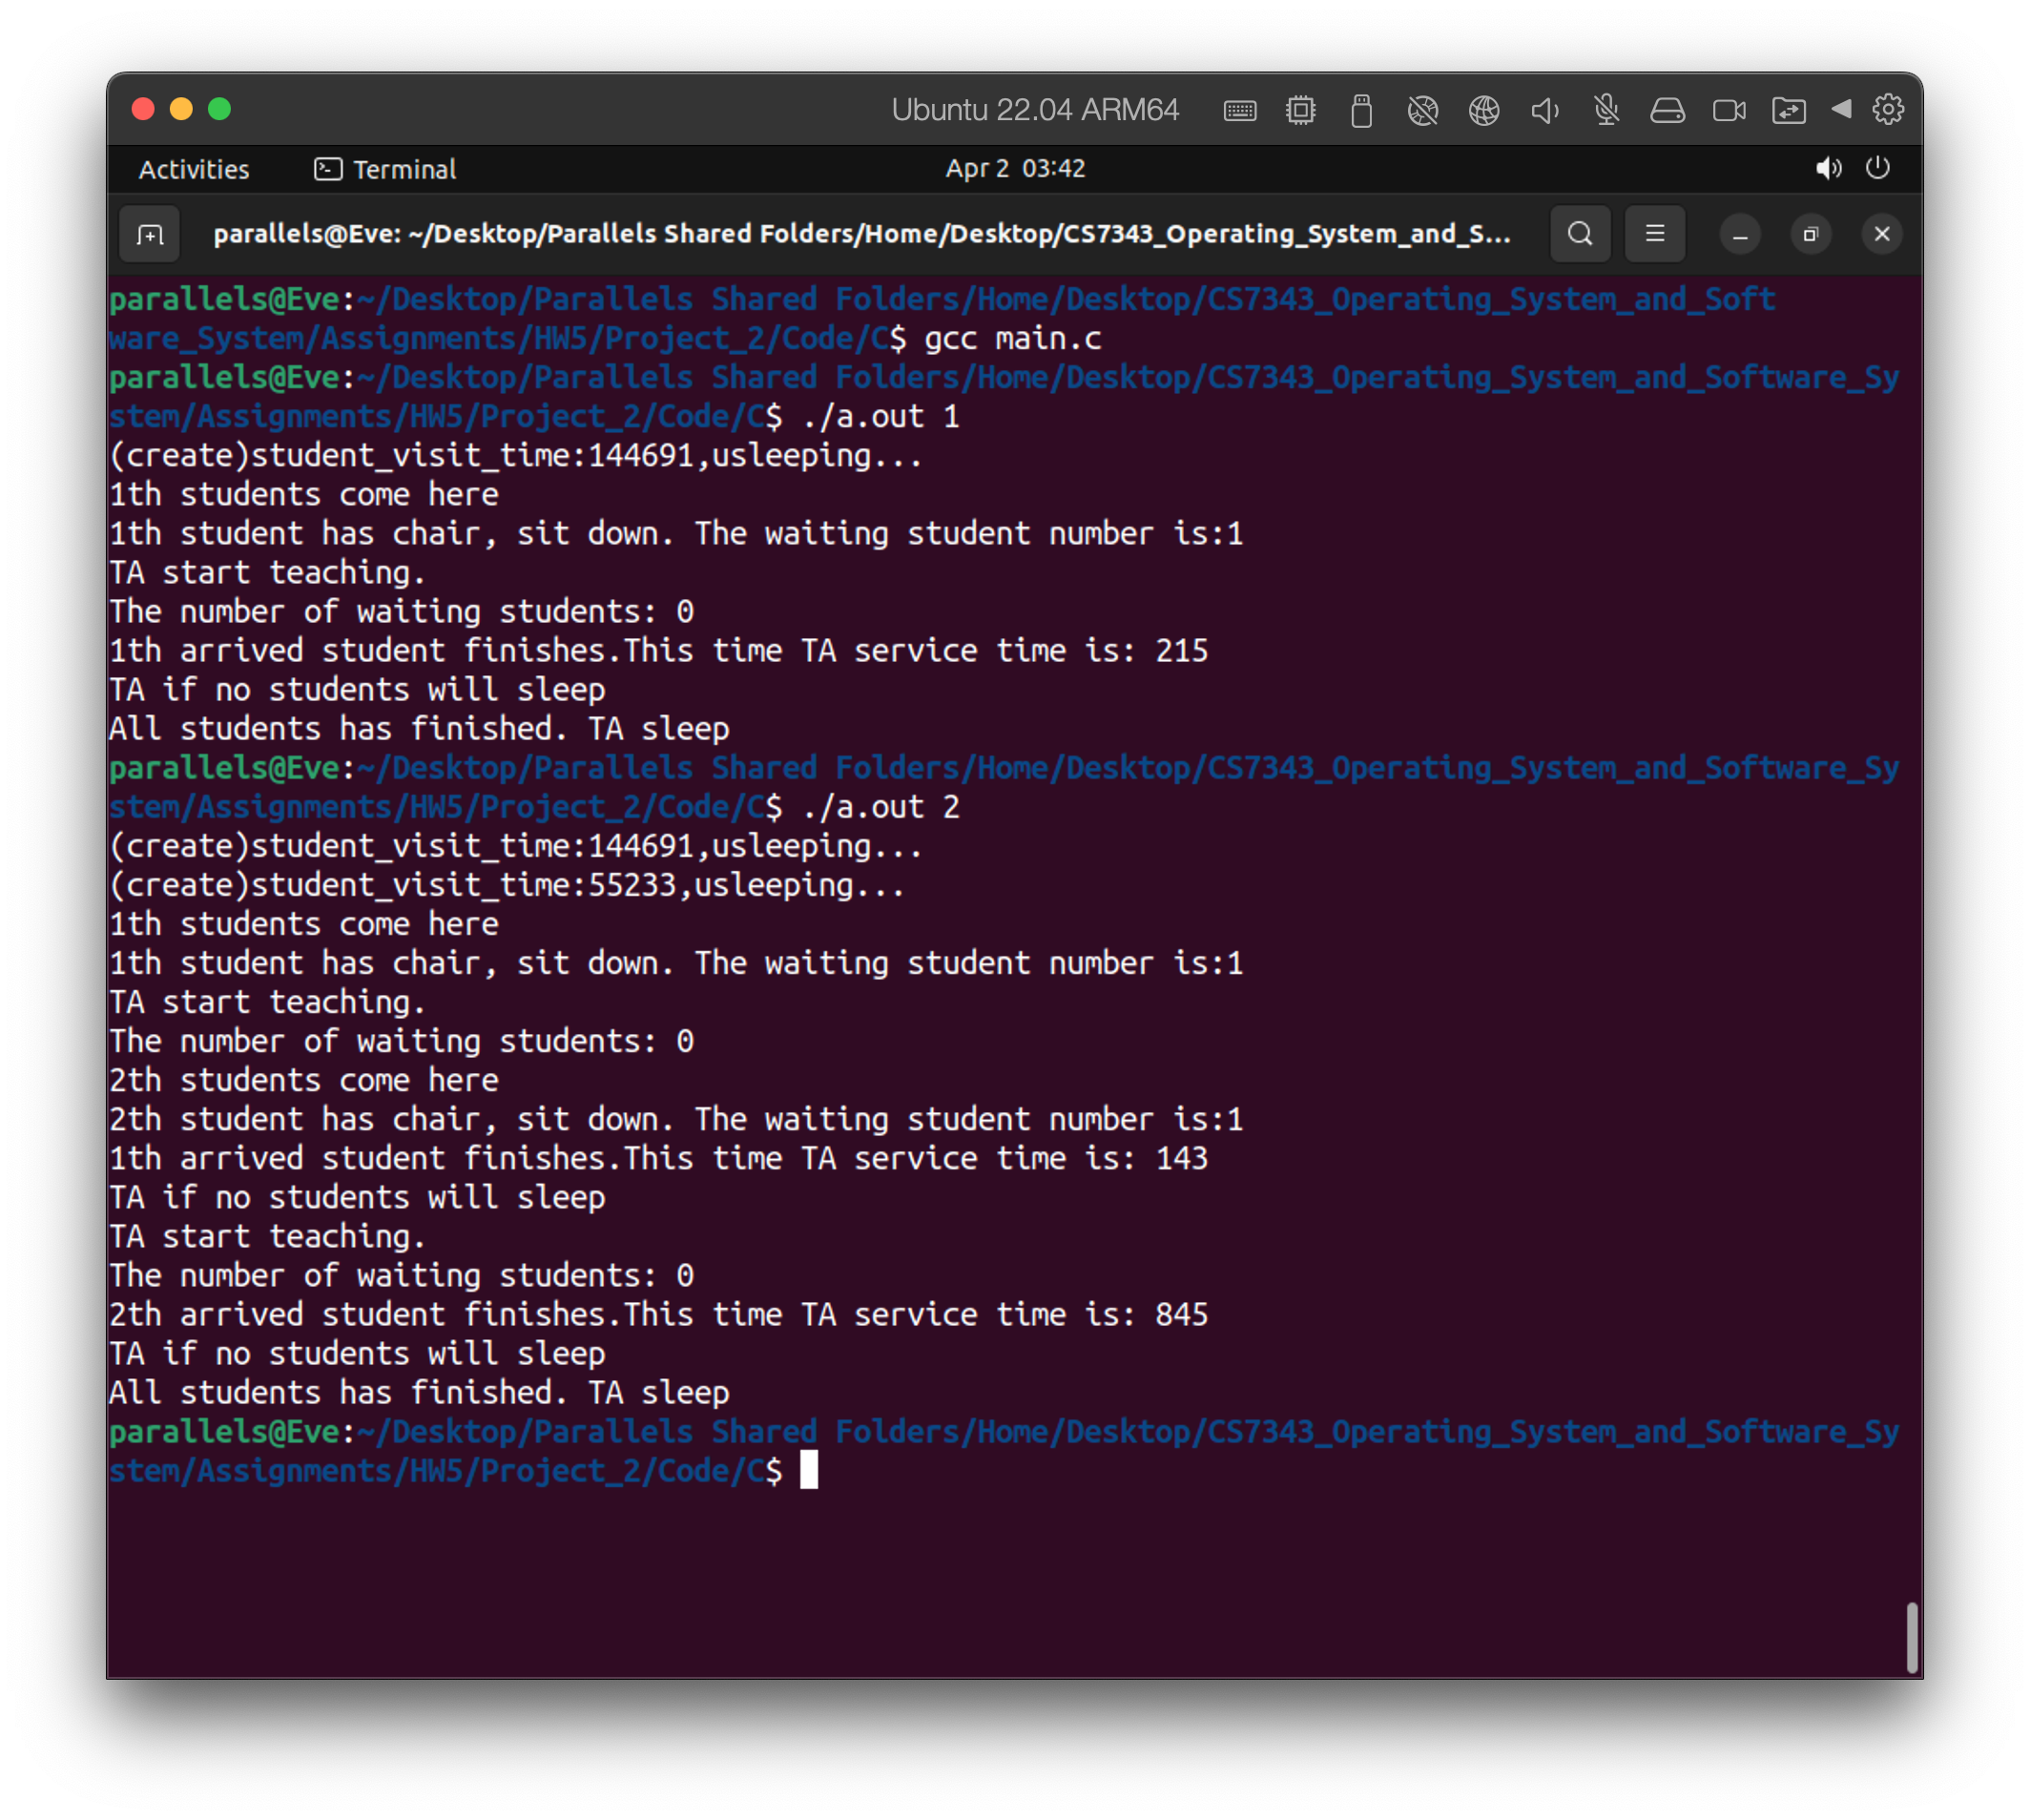
\includegraphics[width=0.9\textwidth]{1.png}
        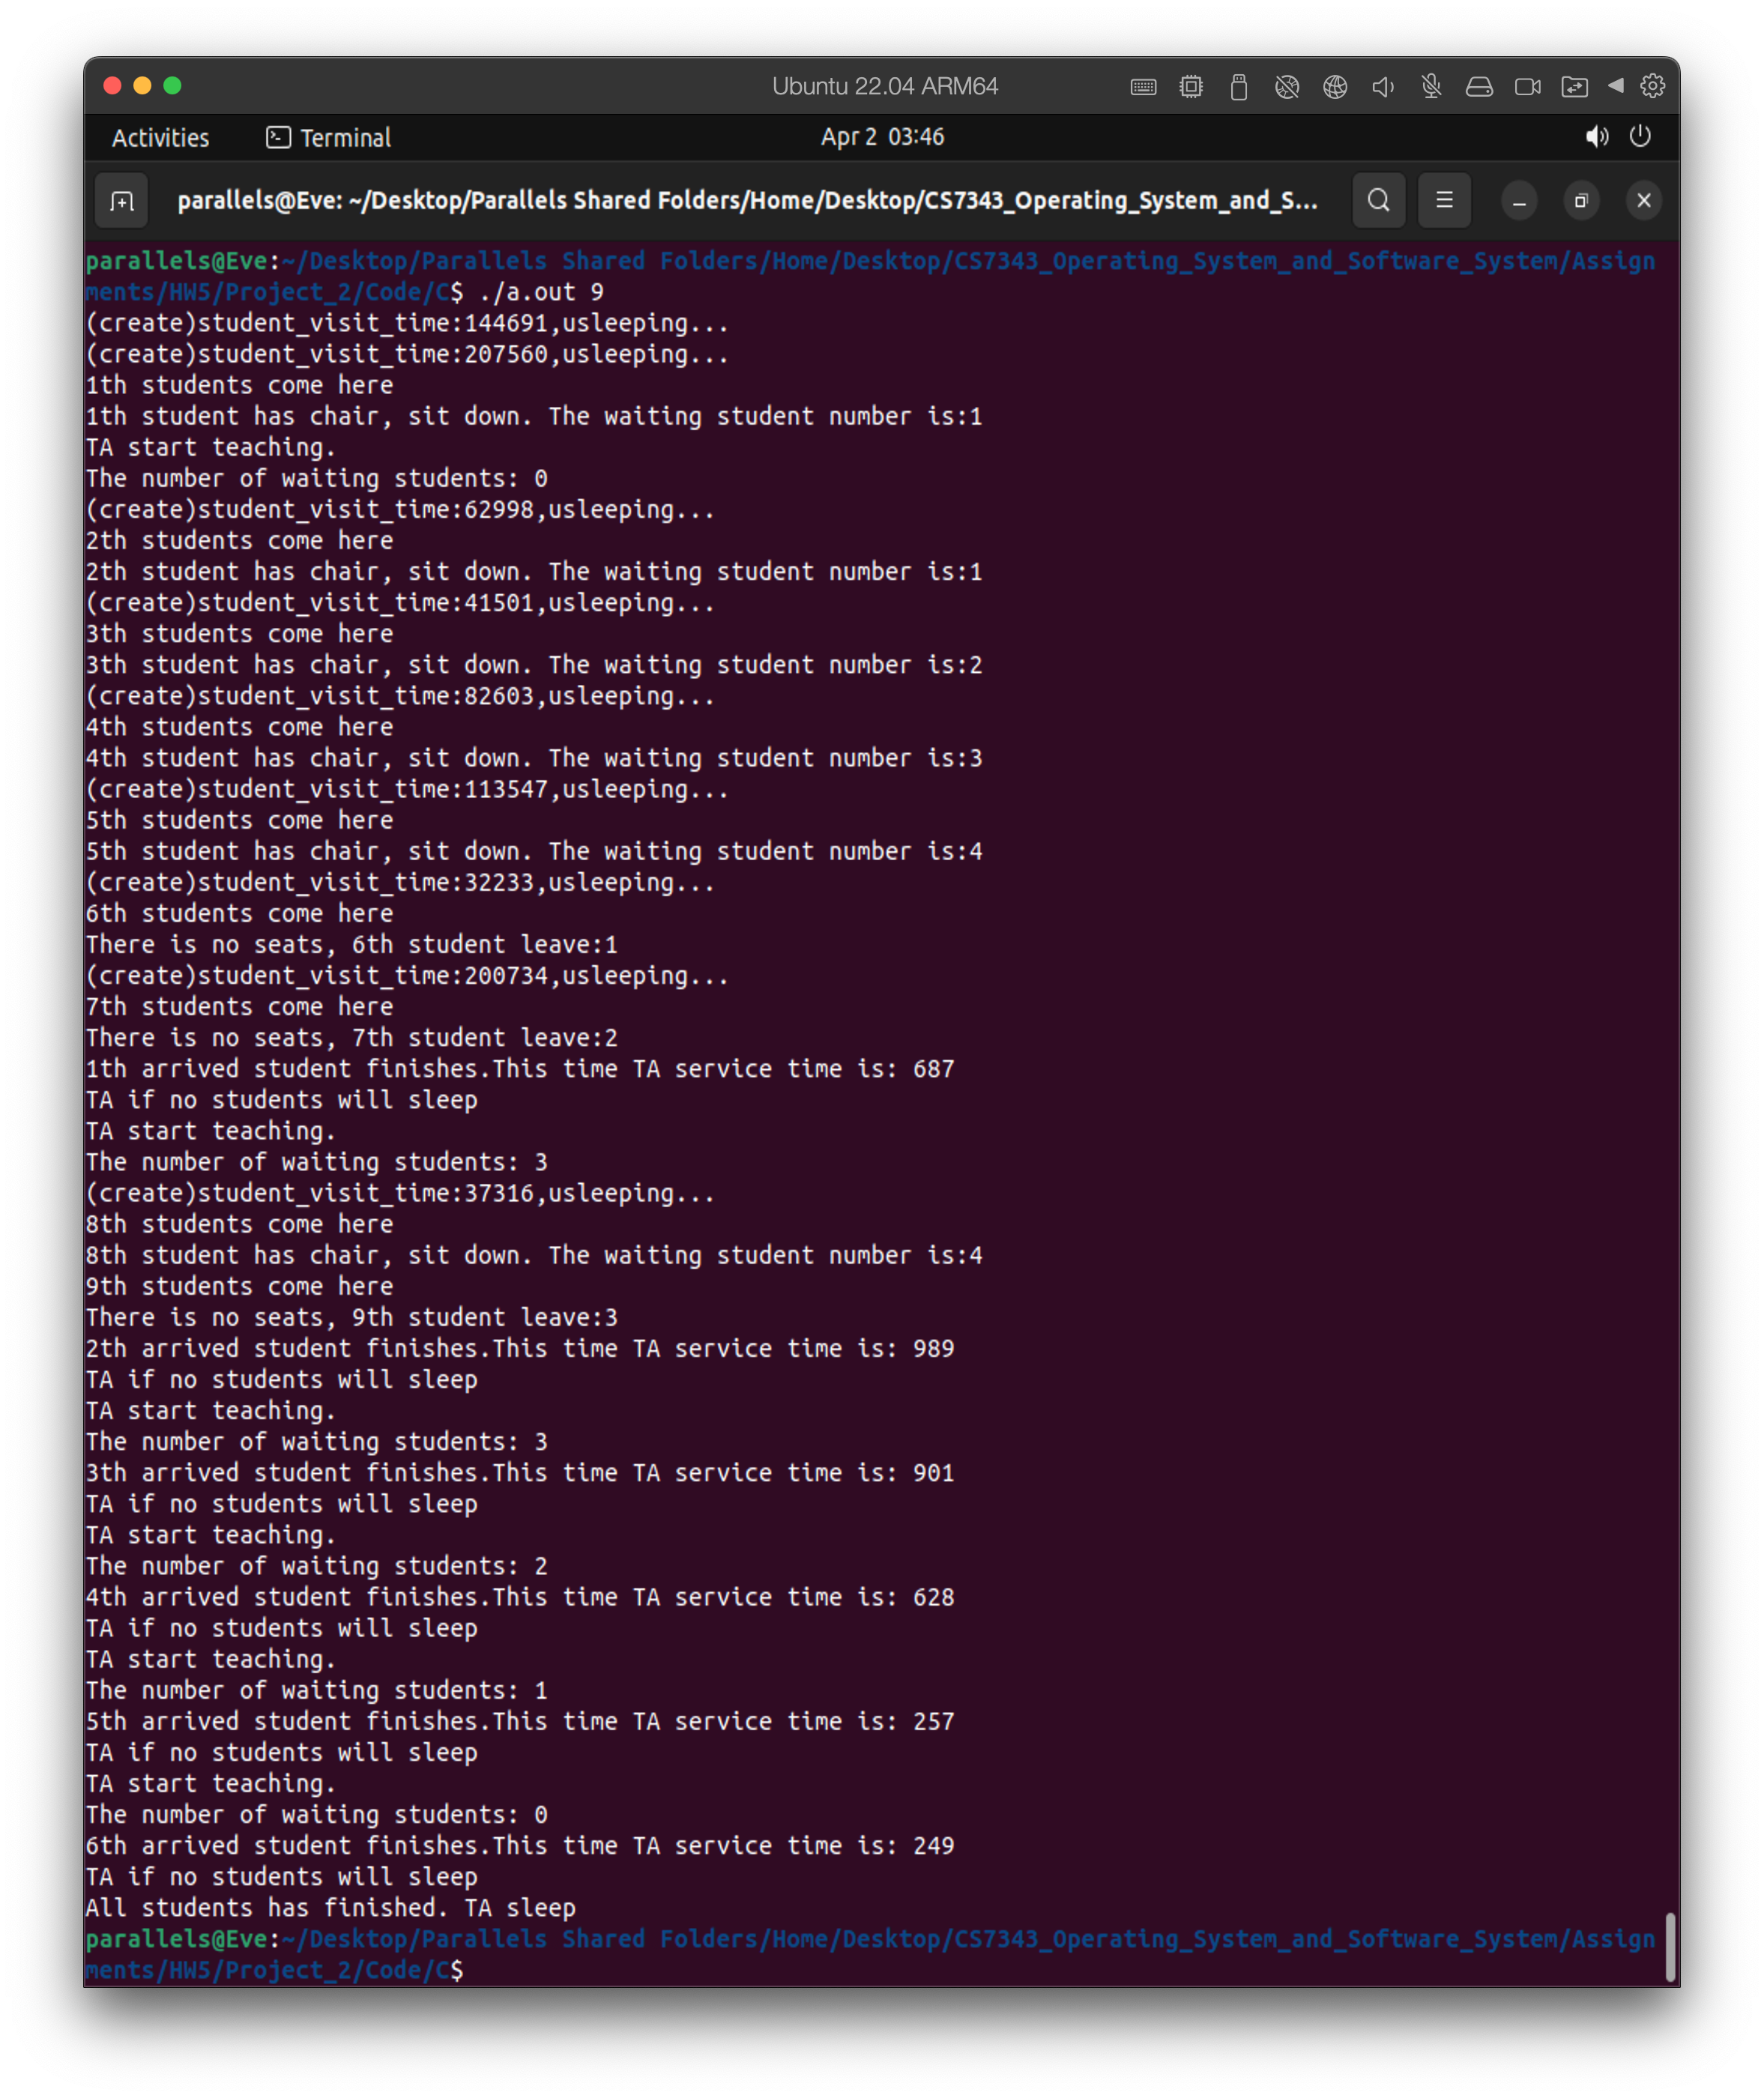
\includegraphics[width=0.9\textwidth]{12.png}
    \end{center}
    
    \end{sol}

    \newpage
    \section*{Project 3--The Dining-Philosophers Problem}
    In Section 7.1.3, we provide an outline of a solution to the dining-philosophers problem using monitors. This project involves implementing a solution to this problem using either POSIX mutex locks and condition variables of Java condition variables. Solutions will be based on the algorithm illustrated in Figure 7.7.\\
    Both implementations will require creating five philosophers, each identified by a number $0\dots 4$. Each philosopher will run as a separate thread. Philosophers alternate between thinking and eating. To simulate both activities, have each thread sleep for a random period between one and three seconds.
    \begin{sol}
    \hspace*{\fill}\\
    \textbf{main.c}:
        \begin{minted}[frame=lines,framesep=2mm,baselinestretch=1.2,fontsize=\footnotesize,linenos]{c}
//
// Created by Eve Liang on 3/26/23.
//
#include <stdio.h>
#include <pthread.h>
#include <unistd.h>
#include <stdlib.h>

/*    p0   p1   p2
        p3   p4
 */


void pickup(int i);
void putdown(int i);
void test(int i);
void *runner(void *param); /* threads call this function */

pthread_mutex_t mutex;
pthread_cond_t cond_var[5];

int eating_number;

// monitor DiningPhilosophers
enum {THINKING, HUNGRY, EATING} state[5];

// pi hungry, pi want to pickup if yes state --> EAT
void pickup(int i){
    pthread_mutex_lock(&mutex);
    state[i] = HUNGRY;
    test(i);
    while (state[i] != EATING) {
        //self[i].wait();
        //printf("Philosopher%d is HUNGRY and waiting to pick up.\n", i);
        pthread_cond_wait(&cond_var[i], &mutex);
    }
    pthread_mutex_unlock(&mutex);
}

// check pi whether can eat
void test(int i){
    if ((state[(i + 4) % 5] != EATING) &&
    (state[i] == HUNGRY) && (state[(i + 1) % 5] != EATING)){
        state[i] = EATING;
        pthread_cond_signal(&cond_var[i]);                    // self[i].signal();
    }
}

// putdown, pi change to think, and check neighbour pi+1, p-1 whether want to pickup
void putdown(int i){
    pthread_mutex_lock(&mutex);
    state[i] = THINKING;
    test((i + 4) % 5);
    test((i + 1) % 5);
    pthread_mutex_unlock(&mutex);
}

int main(int argc, char *argv[]) {
    if (argc != 2){
        fprintf(stderr,"Please use the command format: 
        <the number of philosophers eating times>");
        return -1;
    }
    eating_number = atoi(argv[1]);
    int index[5];

    pthread_t tid[5]; /* the thread identifier */
    pthread_attr_t attr; /* set of the thread attributes */

    /* set the default attributes of the thread */
    pthread_attr_init(&attr);
    // create and initialize a thread's attribute structure

    pthread_mutex_init(&mutex, NULL);

    for (int i = 0; i < 5; i++) {
        state[i] = THINKING;
        pthread_cond_init(&cond_var[i], NULL);
    }

    //  create the thread
    for (int i = 0; i < 5; i++) {
        index[i] = i;
        pthread_create(&tid[i], &attr, runner, &index[i]); // create a new thread
    }

    /* wait for the thread to exit */
    for (int i = 0; i < 5; i++) {
        pthread_join(tid[i], NULL); // Wait for a specific thread to exit4
    }

    return 0;
}

void *runner(void *param){
    int i = *((int *) param);
    int count = 0;
    int time; // sleep for a random period between one and three seconds.
    while (count < eating_number){
        count++;
        printf("Philosopher%d is thinking in %d times.\n", i, count);
        time = rand() % 3 + 1;
        sleep(time);
        printf("Philosopher%d is ending %d times thinking, time is %d seconds\n",
               i, count, time);
        printf("Philosopher%d is hungry now.\n", i);
        pickup(i);
        printf("Philosopher%d is pickup chopsticks and eating in %d times\n", 
               i, count);
        time = rand() % 3 + 1;
        sleep(time);
        printf("Philosopher%d is ending %d times of eating.\n", 
                i, count);
        putdown(i);
        printf("Philosopher%d is put down chopsticks.\n", i);

    }

    pthread_exit(0);
}
        
    \end{minted}
        \textbf{The result}
    \begin{minted}[frame=lines,framesep=2mm,baselinestretch=1.2,fontsize=\footnotesize]{c}
 ./<filename> <The times of philosopher eating>
    \end{minted}
    The result for running of each philosopher only eating one times and two times.
    \begin{center}
        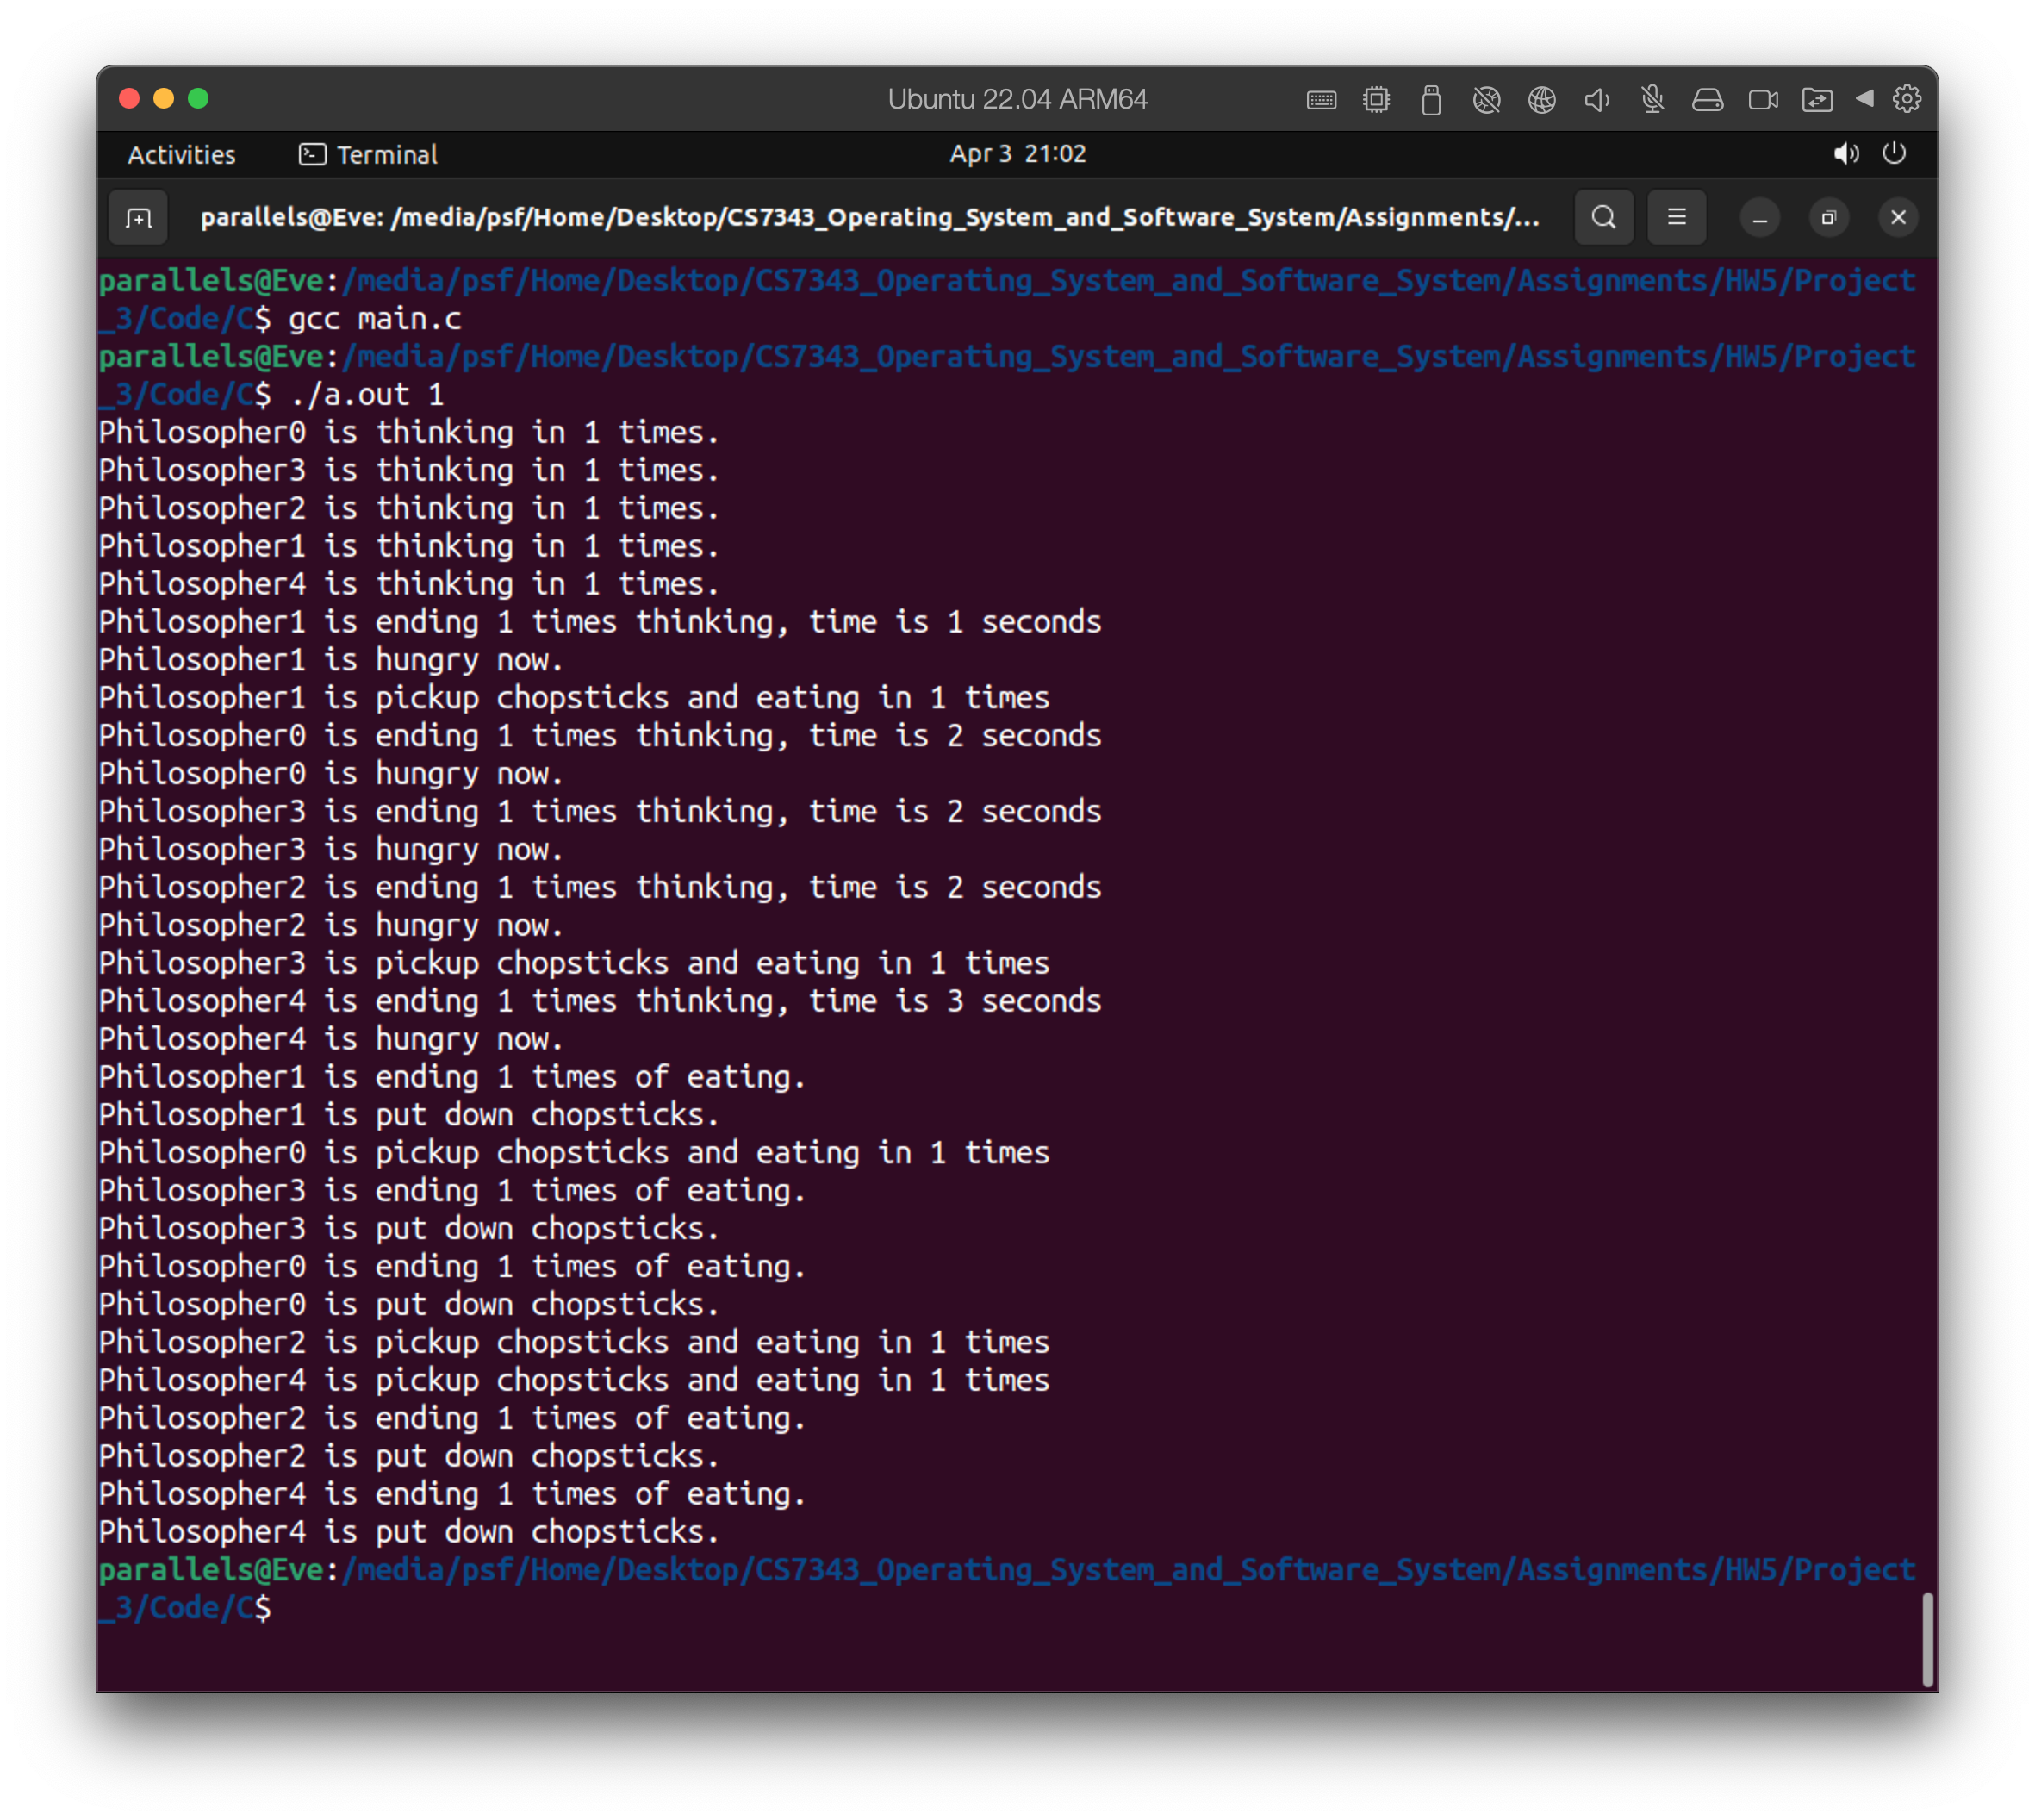
\includegraphics[width=0.9\textwidth]{2.png}
        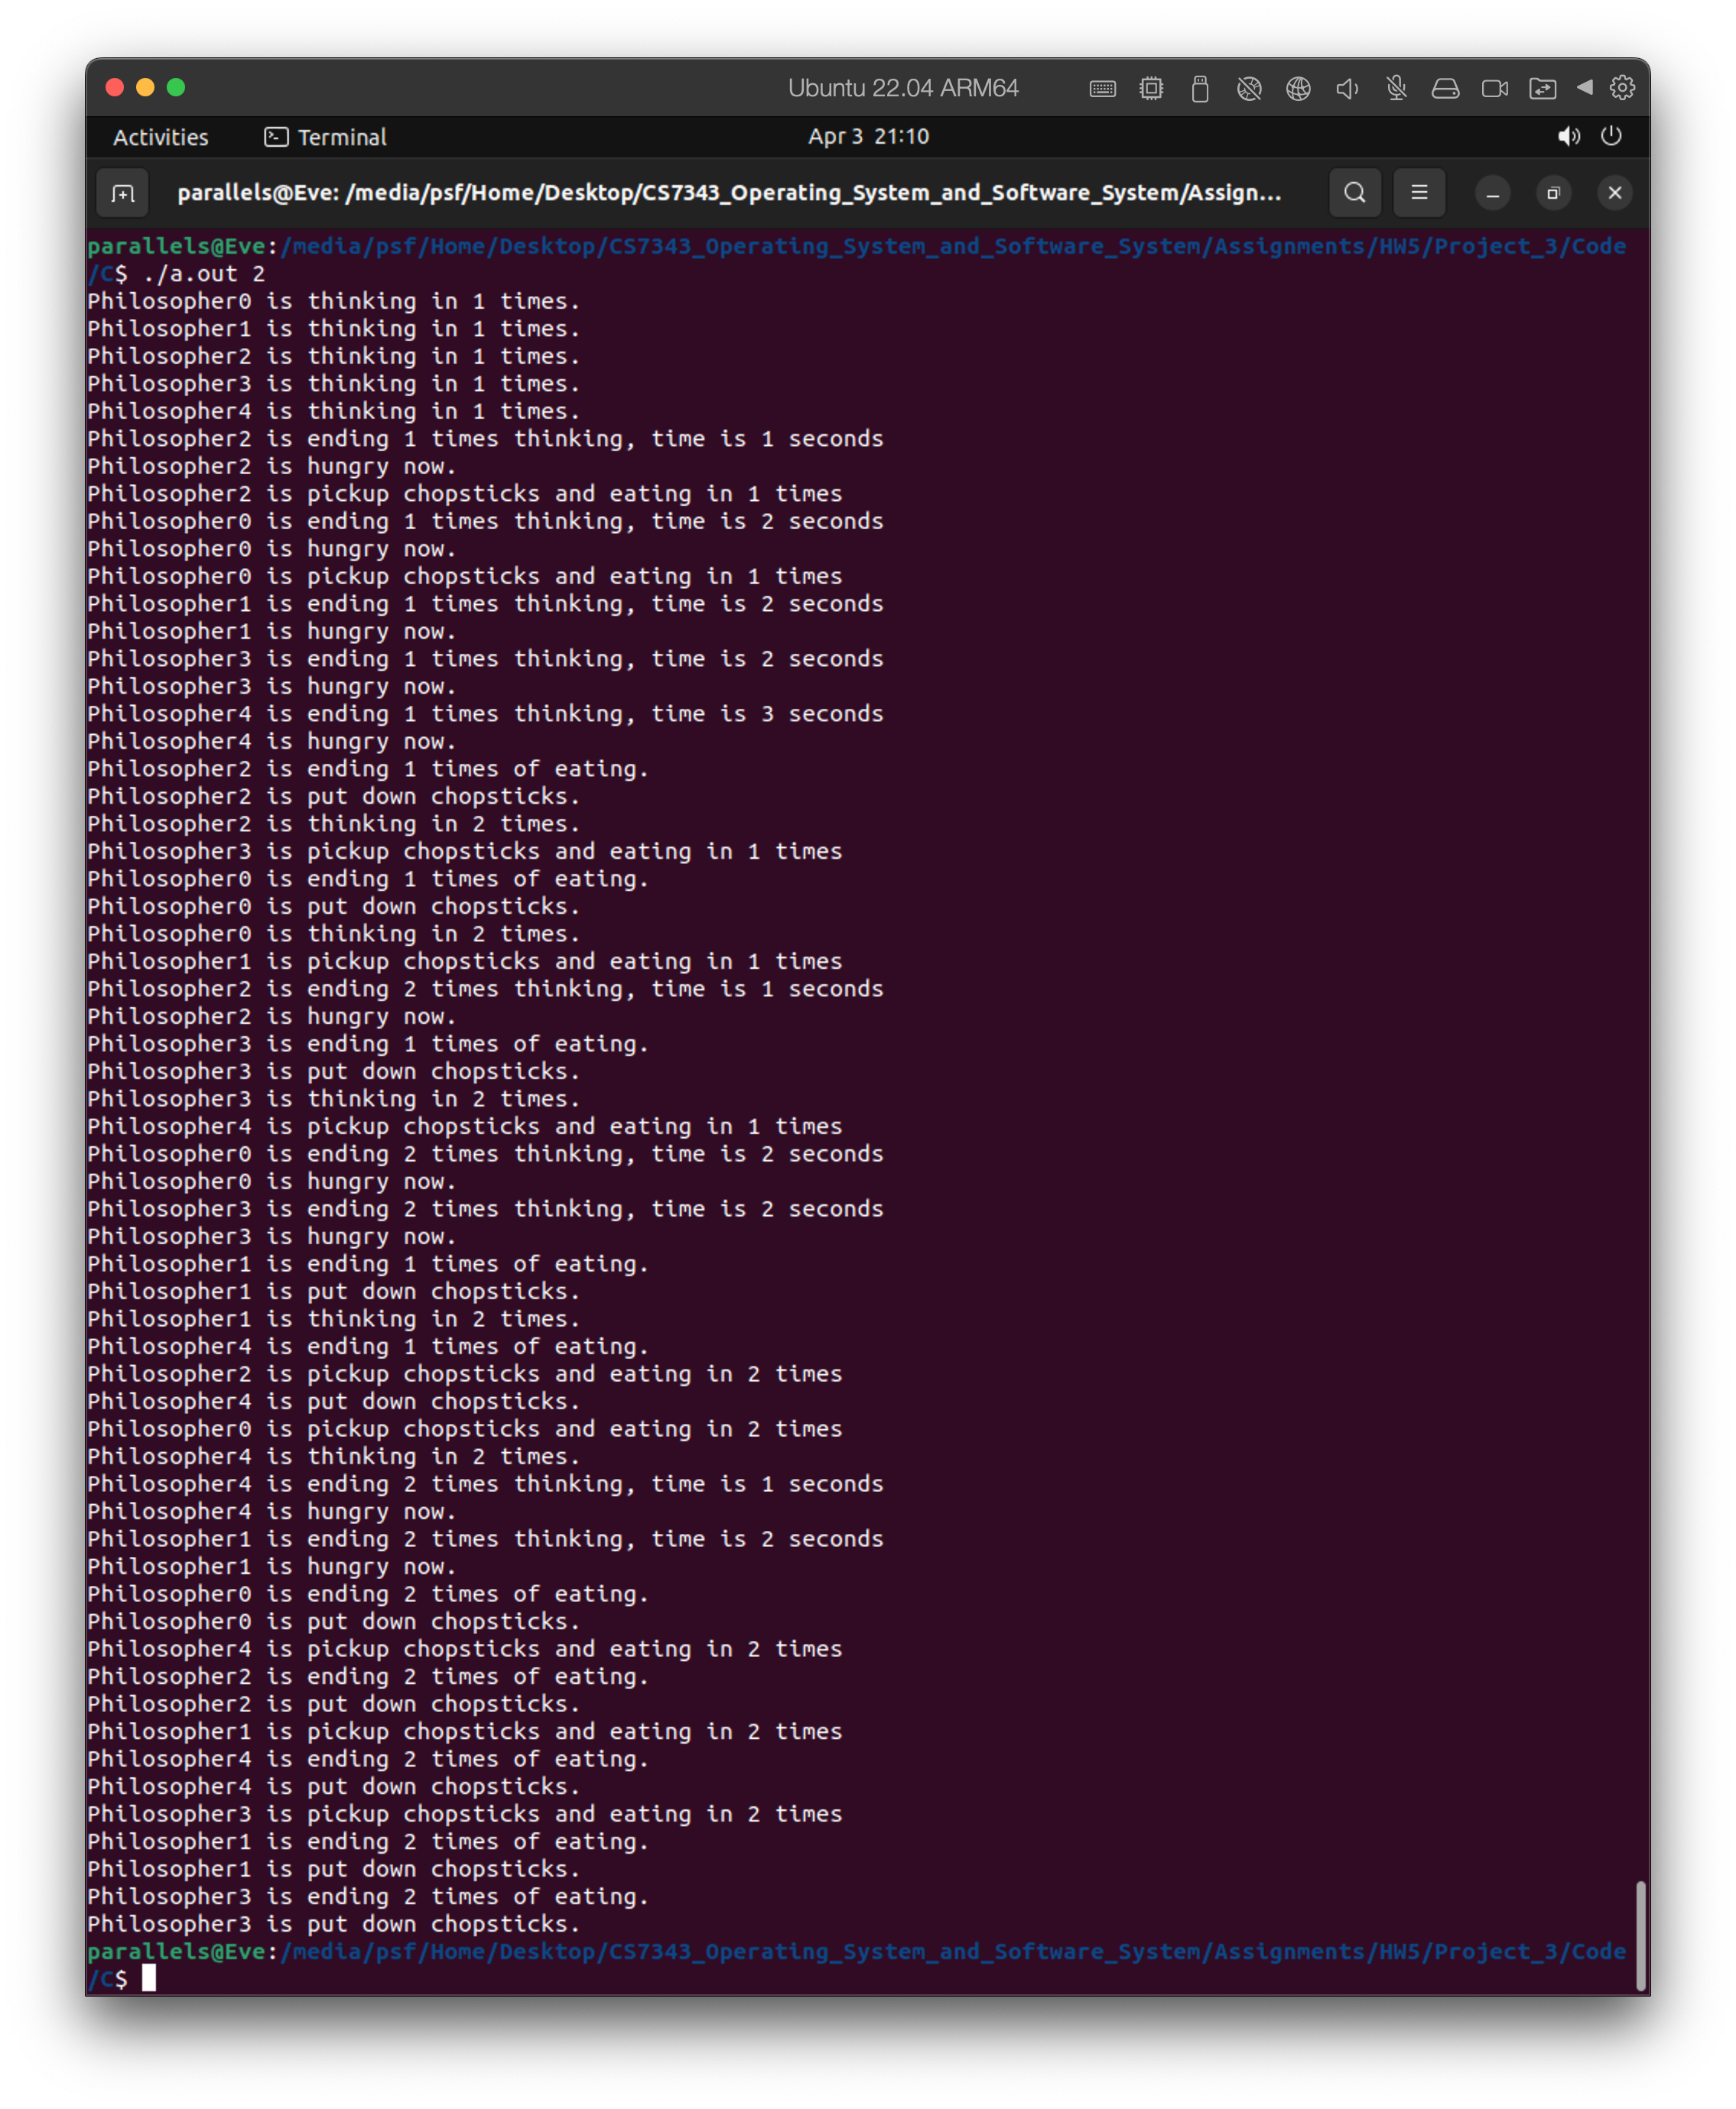
\includegraphics[width=0.9\textwidth]{22.png}
    \end{center}
    \end{sol}


    \newpage
    \section*{Project 4--The Producer-Consumer Problem}
    
    In section 7.1.1, we presented a semaphore-based solution to the producer-consumer problem using a bounded buffer. In this project, you will design a programming solution to the bounded-buffer problem using the producer and consumer processes shown in Figure 5.9 and 5.10. The solution presented in Section 7.1.1 uses three semaphores: empty and full, which count the number of empty and full slots in the buffer, and mutex, which is a binary (or mutual-exclusion) semaphore that protects the actual insertion or removal of items in the buffer. For this project, you will use standard counting semaphores for empty and full and a mutex lock rather than a binary semaphore, to represent mutex. The producer and consumer--running as separate threads--will move items to and from a buffer that is synchronized with the empty, full, and mutex structures. You can solve this problem using either Pthreads or the Windows API.
    \begin{sol}
    \hspace*{\fill}\\
    \begin{enumerate}
        \item[(a)]     \textbf{The buffer:}    buffer.h
    \begin{minted}[frame=lines,framesep=2mm,baselinestretch=1.2,fontsize=\footnotesize,linenos]{c}
// Created by Eve Liang on 3/26/23.
//
/* buffer.h */
/* buffer fix array, statement of item; */
typedef int buffer_item;

/* The definition of the array size */
#define BUFFER_SIZE 5        

/* The operation in the buffer, separately used for 
producer and consumer thread */
int insert_item(buffer_item item);
int remove_item(buffer_item *item);
    \end{minted}

\item[(b)]\textbf{The buffer operations:} buffer.c
    \begin{minted}[frame=lines,framesep=2mm,baselinestretch=1.2,fontsize=\footnotesize,linenos]{c}
// Created by Eve Liang on 3/26/23.
//
#include "buffer.h"

#include <pthread.h>
#include <semaphore.h>

/* the buffer */
buffer_item buffer[BUFFER_SIZE];

pthread_mutex_t mutex;   /*pthread mutex lock*/

/* semaphore data type */
sem_t empty; // buffer empty
sem_t full;  // buffer full

int insertIndex = 0;
int removeIndex = 0;

/* threads function */
void *producer(void *param);
void *consumer(void *param);


int insert_item(buffer_item item){
    /* insert item into buffer
    return 0 if successful, otherwise
    return -1 indicating an error condition */

    /* produce an item in next_produced */
    sem_wait(&empty); // wait(empty)
    pthread_mutex_lock(&mutex); // wait(mutex)

    /* add next_produced to the buffer */
    buffer[insertIndex] = item;
    insertIndex++;
    insertIndex = insertIndex % BUFFER_SIZE;

    pthread_mutex_unlock(&mutex); // signal(mutex)
    sem_post(&full); // signal(full)

    return 0;
}

int remove_item(buffer_item *item){
    /* remove an object from buffer
    placing it in item
    return 0 if successful, otherwise
    return -1 if indicating an error condition */
    sem_wait(&full);   // wait(full)
    pthread_mutex_lock(&mutex);  // wait(mutex)

    /* remove an item from buffer to next_consumed */
    *item = buffer[removeIndex];
    buffer[removeIndex] = -1;
    removeIndex++;
    removeIndex = removeIndex % BUFFER_SIZE;

    pthread_mutex_unlock(&mutex);  // signal(mutex)
    sem_post(&empty);       // signal(empty)

    /* consume the item in next_consumed */
    return 0;
}
        
    \end{minted}

    \item[(c)] \textbf{Main: } main.c 
        \begin{minted}[frame=lines,framesep=2mm,baselinestretch=1.2,fontsize=\footnotesize,linenos]{c}
// Created by Eve Liang on 3/26/23.
//
#include "buffer.h"
#include <stdio.h>
#include <stdlib.h>
#include <pthread.h>
#include <semaphore.h>
#include <unistd.h>

#include "pcthreads.c"
#include "buffer.c"

#define TRUE 1

int main(int argc, char*argv[]) {
    /*  The `main()` function will be passed three parameters on the command line:
        1. How long to sleep before terminatin
        2. The number of producer threads
        3. The number of consumer threads
     */

    /* 1. Get command line arguments argv[1], argv[2], argv[3] */
    int sleepTime;
    int n_producer;  // n_producer thread
    int n_consumer;  // n_consumer thread
    int i, j;
    if (argc != 4) {
        fprintf(stderr,
        "Please use the command format: <How long to sleep before terminatin>
        <producer number> <consumer number>");
        return -1;
    }

    sleepTime = atoi(argv[1]);
    n_producer = atoi(argv[2]);
    n_consumer = atoi(argv[3]);

    /* 2. Initialize buffer */
    pthread_mutex_init(&mutex, NULL);
    sem_init(&empty, 0, BUFFER_SIZE);
    sem_init(&empty, 0, BUFFER_SIZE);
    srand(time(0));

    /* 3. Create producer thread(s) */
    for (i = 0; i < n_producer; i++) {
        pthread_t tid;
        pthread_attr_t attr;
        pthread_attr_init(&attr);
        pthread_create(&tid, &attr, producer, NULL);
    }

    /* 4. Create n_consumer thread(s) */
    for (j = 0; j < n_consumer; j++) {
        pthread_t tid;
        pthread_attr_t attr;
        pthread_attr_init(&attr);
        pthread_create(&tid, &attr, consumer, NULL);
    }

    /* 5. Sleep */
    sleep(sleepTime);

    /* 6 Exit */
    return 0;
}
        
    \end{minted}
    \item[(d)] \textbf{The Producer and Consumer Threads:} pcthreads.c
            \begin{minted}[frame=lines,framesep=2mm,baselinestretch=1.2,fontsize=\footnotesize,linenos]{c}
// Created by Eve Liang on 3/26/23.
//
#include "buffer.h"
#include <stdio.h>
#include <stdlib.h>
#include <pthread.h>
#include <semaphore.h>
#include <unistd.h>

#include "pcthreads.c"
#include "buffer.c"

#define TRUE 1

int main(int argc, char*argv[]) {
    /*  The `main()` function will be passed three parameters on the command line:
        1. How long to sleep before terminatin
        2. The number of producer threads
        3. The number of consumer threads
     */

    /* 1. Get command line arguments argv[1], argv[2], argv[3] */
    int sleepTime;
    int n_producer;  // n_producer thread
    int n_consumer;  // n_consumer thread
    int i, j;
    if (argc != 4) {
        fprintf(stderr,
                "Please use the command format: <How long to sleep before terminatin> <producer number> <consumer number>");
        return -1;
    }

    sleepTime = atoi(argv[1]);
    n_producer = atoi(argv[2]);
    n_consumer = atoi(argv[3]);

    /* 2. Initialize buffer */
    pthread_mutex_init(&mutex, NULL);
    sem_init(&empty, 0, BUFFER_SIZE);
    sem_init(&empty, 0, BUFFER_SIZE);
    srand(time(0));

    /* 3. Create producer thread(s) */
    for (i = 0; i < n_producer; i++) {
        pthread_t tid;
        pthread_attr_t attr;
        pthread_attr_init(&attr);
        pthread_create(&tid, &attr, producer, NULL);
    }

    /* 4. Create n_consumer thread(s) */
    for (j = 0; j < n_consumer; j++) {
        pthread_t tid;
        pthread_attr_t attr;
        pthread_attr_init(&attr);
        pthread_create(&tid, &attr, consumer, NULL);
    }

    /* 5. Sleep */
    sleep(sleepTime);

    /* 6 Exit */
    return 0;
}
\end{minted}

        \end{enumerate}
    \textbf{The result}
    \begin{minted}[frame=lines,framesep=2mm,baselinestretch=1.2,fontsize=\footnotesize]{c}
 ./<filename> <execute time> <producers number> <consumer number>
    \end{minted}
    The result for running the for 8 seconds with 2 producer and 2 consumer.
    \begin{center}
        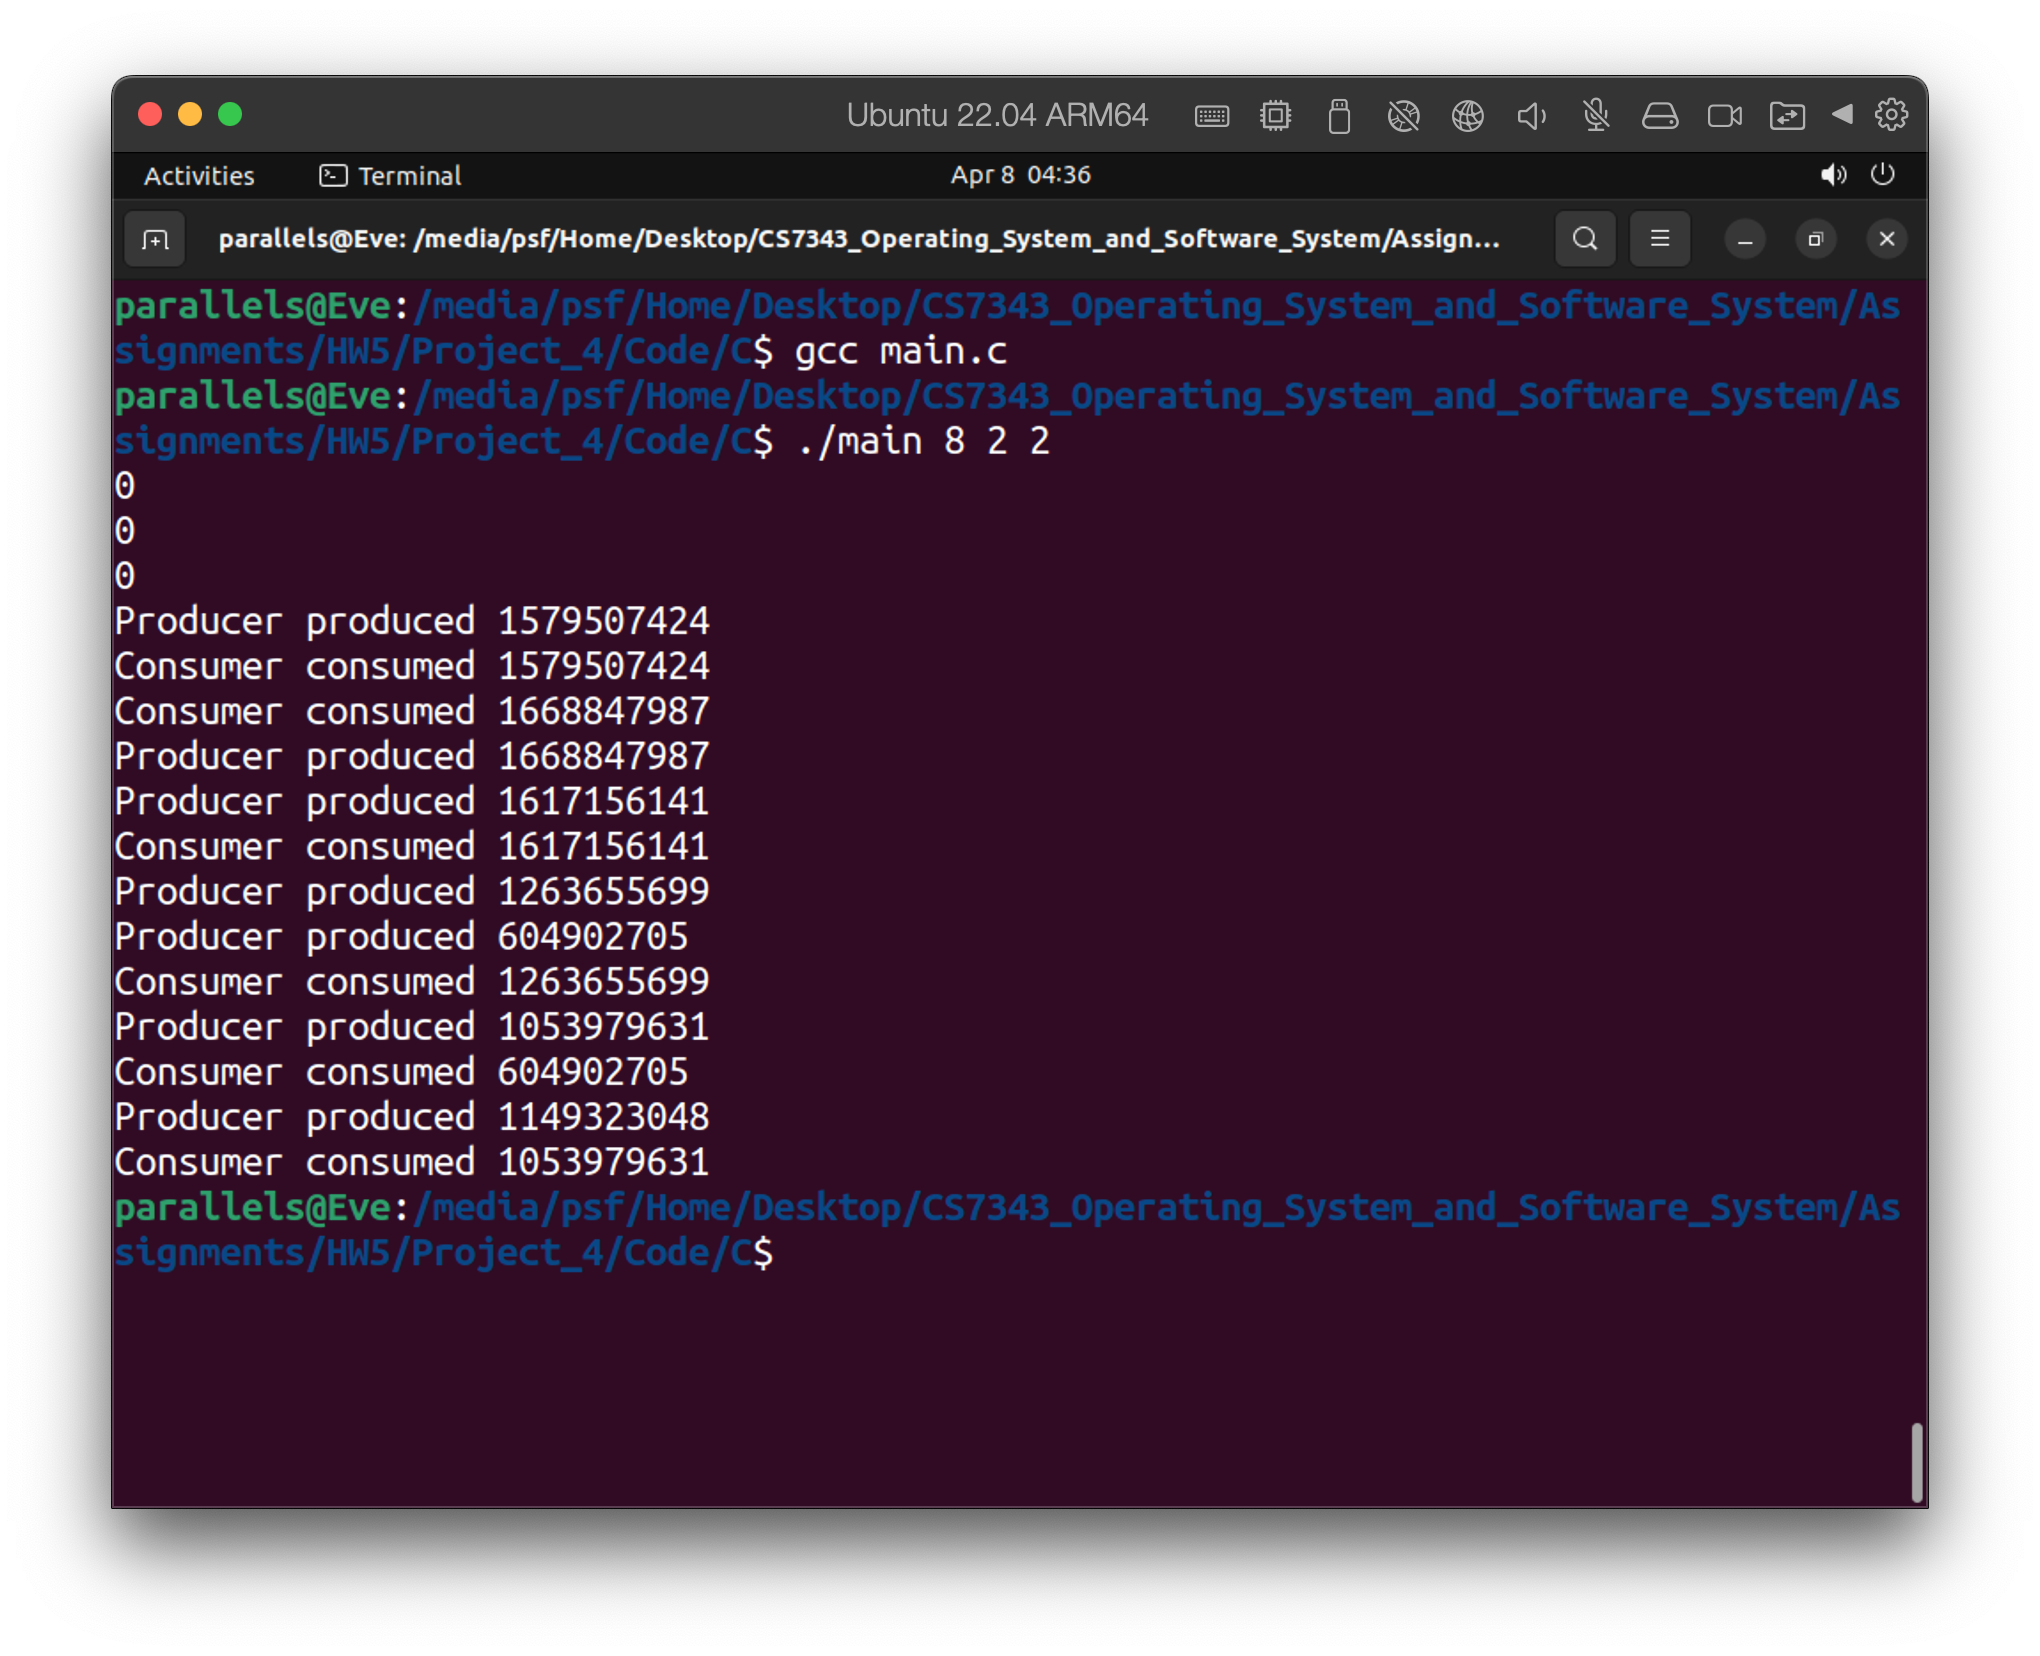
\includegraphics[width=0.9\textwidth]{3.png}
    \end{center}
    \end{sol}
    More code detail can see in the source code of the projects.

\end{document}
